\section{\label{s:verify}System Setup and Verification}

\subsection{\label{ss:corrRange}Correction Range}

% FROM THESIS
Figure \ref{f:phaseVsAmpVoltage} shows the measured mean phase shift in the 
downstream phase monitor across the full \(\pm2\)~V input range of the 
amplifier. Constant DAC outputs in 17 steps between -4095 counts (-2~V) and 
+4095 counts (+2~V) were used to drive the amplifier. For each amplifier input 
voltage 100 beam pulses were acquired in interleaved mode in order to reduce 
the sensitivity to any drifts in beam phase between data points. The phase 
plotted in Figure~\ref{f:phaseVsAmpVoltage} is the difference between the 50 
beam pulses with the DAC output enabled (non-zero amplifier input) and the 50 
beam pulses with the DAC output disabled (0~V amplifier input).
At the maximum amplifier input voltage of \(2\)~V the phase is shifted by 
\(5.5\pm0.3^\circ\). The fitted phase shift per Volt input is 
\(3.5\pm0.1^\circ\) in the \(\pm1.2\)~V linear range of the amplifier.
% /FROM THESIS

\begin{figure}
  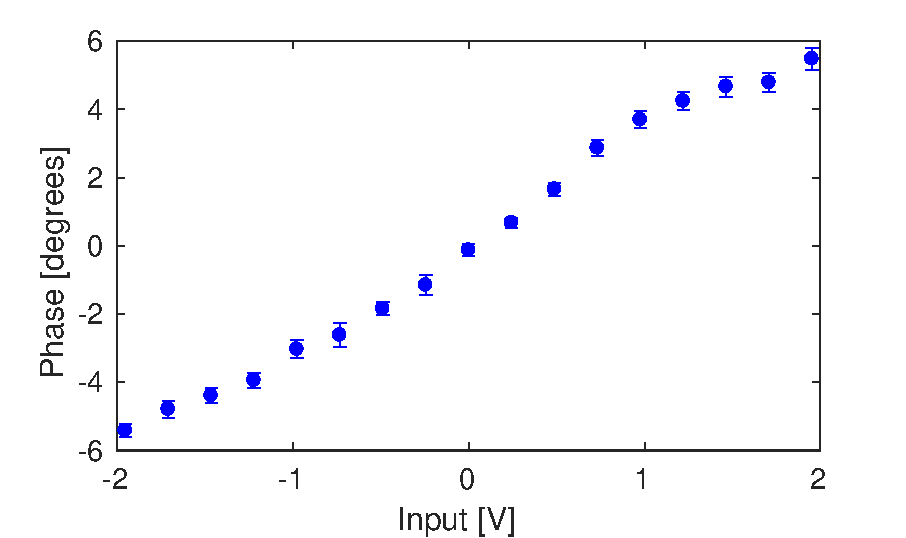
\includegraphics[width=\columnwidth]{corrRange} 
  \caption{\label{f:corrRange}
  }
\end{figure}

The measured correction range is shown in Fig.\ref{f:corrRange}.
Correction range agrees with expected range

Correction shape

% FROM THESIS
In the central region of the pulse all three traces have the same shape as 
expected. The upstream phase and DAC output should be close to identical by 
definition, as the calculated correction output is only dependent on the input 
phase, but this verifies the functionality of the FONT5a board correction 
algorithm and firmware. The agreement in shape of the downstream phase shift is 
a significant achievement, and verifies the linearity of the amplifier output, 
kicker response and optics for a varying input voltage. This result 
demonstrates that everything is in place for the PFF prototype to flatten 
variations in the downstream phase and to reduce the downstream phase jitter.

The agreement in shape holds for times between around 900~ns and 1375~ns as 
indicated on the figure, and this defines a 475~ns portion of the pulse within 
which the applied correction should be close to optimal. Outside this range the 
large phase sag along the pulse leads 
to the correction being saturated -- the maximum possible DAC output 
(2~V) is applied and the shape can no longer be corrected. It can also
be seen that the measured downstream phase shift saturates earlier than
the applied DAC output. This is because the amplifier begins to 
saturate at input voltages below 2~V, as seen in Figure~\ref{f:AmpOutvsDAC}.
% /FROM THESIS

\subsection{\label{ss:corrShape}Correction Shape}

The PFF system removes intra-pulse phase variations as well as inter-pulse 
variations. 

The input upstream phase, calculated DAC output and the observed difference in 
the downstream phase resulting from the applied kick are all shown. The 
downstream phase trace shows the difference between subsequent pulses with the 
correction on and off (using the interleaved correction mode). 
Each trace is scaled, aligned in time and sign flipped where appropriate to 
make a comparison between the shapes easier.

In the central region of the pulse all three traces have the same shape as 
expected. This verifies the linearity of the amplifier output, kicker response 
and optics for a varying input voltage. This result demonstrates that 
everything is in place for the PFF prototype to flatten variations in the 
downstream phase and to reduce the downstream phase jitter.

The agreement in shape holds for times between around 900~ns and 1375~ns as 
indicated on the figure, and this defines a 475~ns portion of the pulse within 
which the applied correction should be close to optimal. Outside this range the 
large phase sag along the pulse leads 
to the correction being saturated -- the maximum possible DAC output 
(2~V) is applied and the shape can no longer be corrected. It can also
be seen that the measured downstream phase shift saturates earlier than
the applied DAC output. This is because the amplifier begins to 
saturate at input voltages below 2~V, as seen in Figure~\ref{f:AmpOutvsDAC}.

\begin{figure}
 \centering
  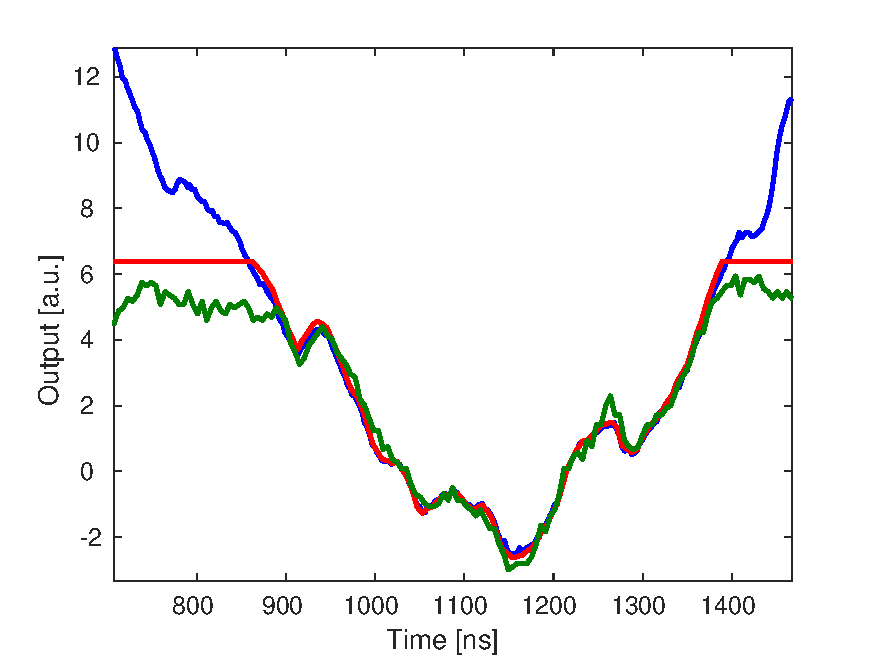
\includegraphics[width=0.6\columnwidth]{pffKickShape} 
  \caption{\label{f:pffKickShape}
  }
\end{figure}

\subsection{\label{ss:orbClos}Orbit Closure}

\begin{figure}
 \centering
  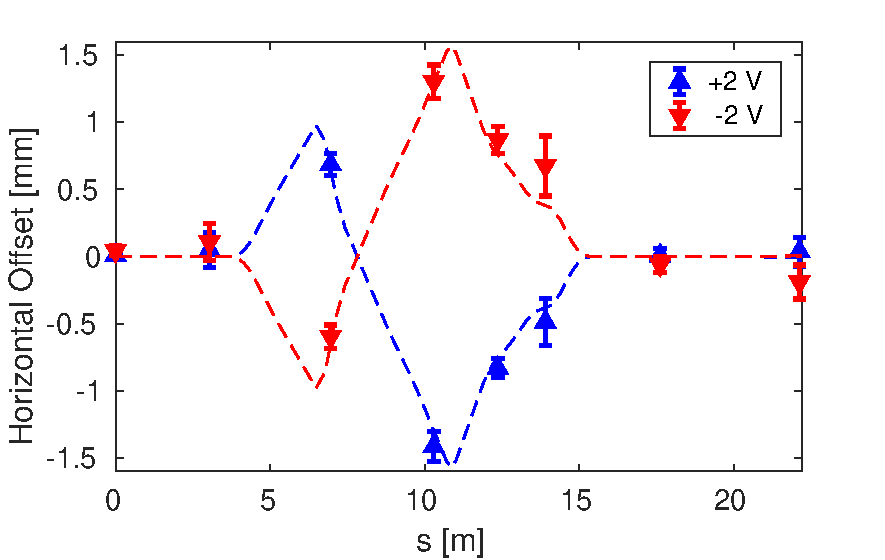
\includegraphics[width=0.6\columnwidth]{orbClos}% Here is 
  %how to 
  %import EPS art
  \caption{\label{f:orbClos}
  }
\end{figure}

Fig.~\ref{f:orbClos} shows the orbit closure measured in the BPMs in and around 
the correction chicane. The BPM orbit is compared to the expected trajectory in 
the nominal optics for the chicane. The measurement and the model are in good 
agreement. A maximum horizontal offset of 1.5~mm inside the chicane is reduced 
to less than 0.1~mm after the chicane.

\subsection{\label{ss:timing}Correction Timing}

To be able to correct intra-pulse phase variations the arrival of the amplifier 
drive voltage at the kicker strips must be precisely synchronised with the 
arrival time of the beam. The correction timing is controlled by the 
feedforward controller and has been optimised with beam based measurements, as 
presented here.

\begin{figure}
 \centering
  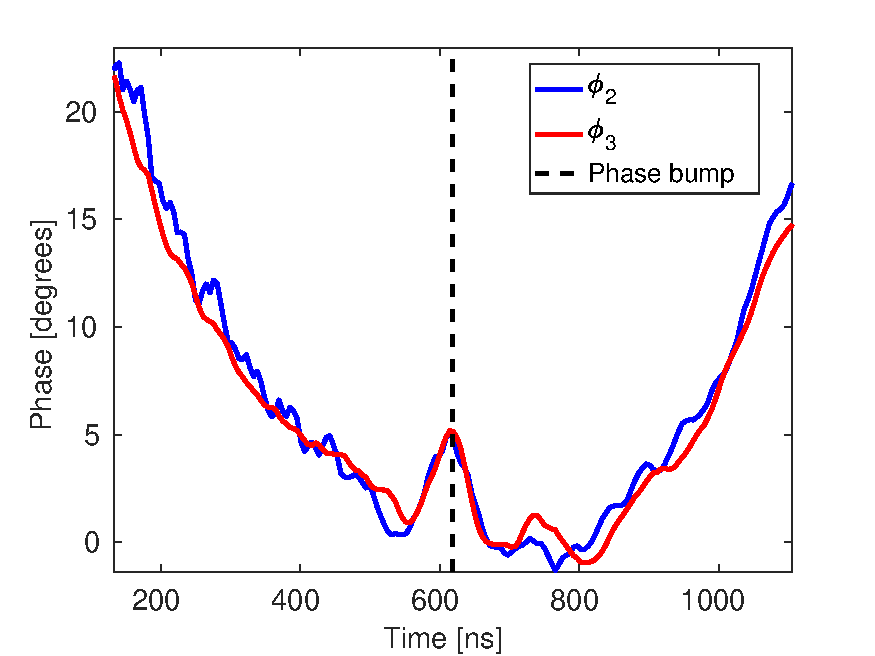
\includegraphics[width=0.5\columnwidth]{bumpMon2Mon3}% Here is 
  %how to 
  %import EPS art
  \caption{\label{f:bumpMon2Mon3} bumpMon2Mon3
  }
\end{figure}

The waveforms of the klystrons were changed to produce a clear phase bump in 
the 
centre of the beam pulse. The bump is clearly visible in both \(\phi_1\) and 
\(\phi_3\), as shown in Fig.~\ref{f:bumpMon2Mon3}. This feature was used to 
determine the necessary delay in the controller output in order to align the 
PFF correction (the kicker voltage) with the beam. 

\begin{figure}
 \centering
  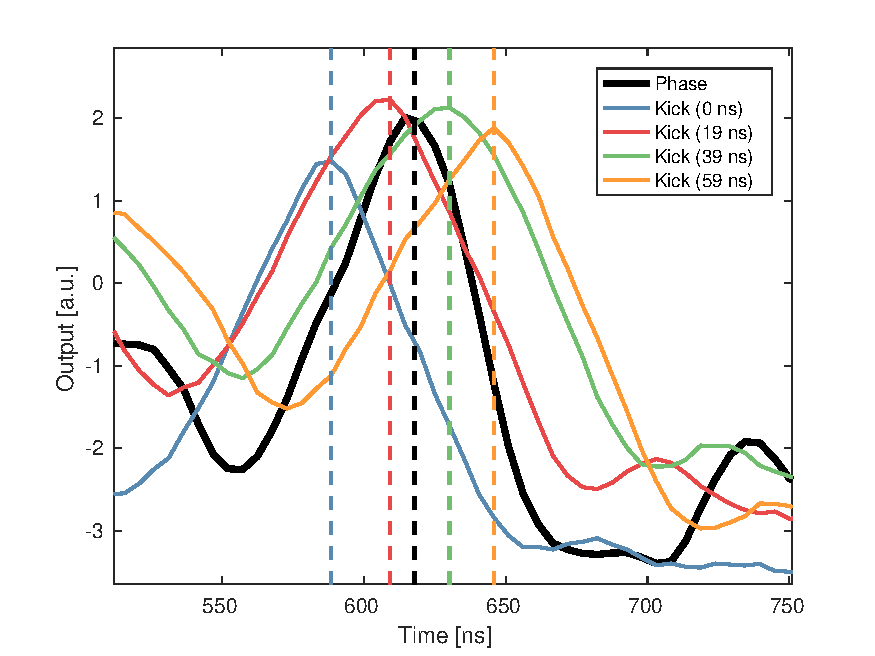
\includegraphics[width=0.6\columnwidth]{absDelay_zoom}% Here is 
  %how to 
  %import EPS art
  \caption{\label{f:absDelay_zoom} absDelay\_zoom
  }
\end{figure}

The PFF correction was applied in interleaved mode. The phase shift at 
\(\phi_3\) caused by the PFF system can then be calculated by taking the 
difference between the `PFF On' and `PFF Off' pulses in the dataset. For the 
optimal system setup this difference should be identical to the initial (`PFF 
Off') phase but with opposite sign.

Fig.~\ref{f:absDelay_zoom} shows the difference (labelled `kick') compared to 
the initial phase for four different controller output delays, zoomed in to the 
region of the pulse with the added phase bump. The differences are sign flipped 
and scaled to facilitate comparisons with the initial phase. Dashed lines 
indicate the time of the phase bump peak in each case. 

\begin{figure}
 \centering
  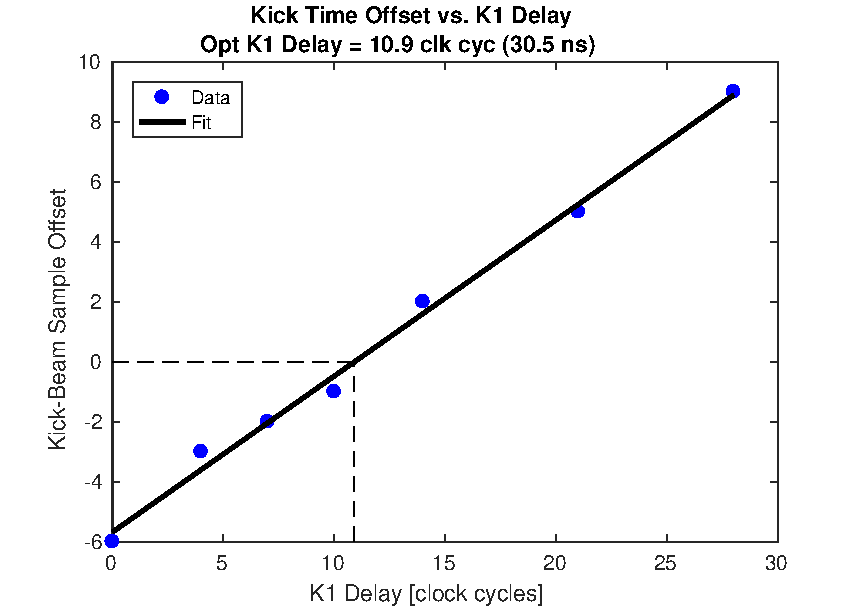
\includegraphics[width=0.6\columnwidth]{OptDelayFit}% Here is 
  %how to 
  %import EPS art
  \caption{\label{f:OptDelayFit} OptDelayFit
  }
\end{figure}

With the correction applied as soon as possible (`Kick 0 ns', blue) the phase 
bump in the applied kick arrives early, at 588~ns in the figure compared to 
618~ns for the initial phase. This proves the PFF system meets the latency 
requirements, with a total system latency of around 350~ns compared to the 
380~ns beam time of flight. As the output delay from the controller is 
increased, the phase bump in the applied kick overlaps and then trails its 
location in the initial phase. Fitting the difference in the peak positions vs. 
the output delay yields an optimal controller delay of \(31\pm4\)~ns 
(Fig.~\ref{f:OptDelayFit}).

\begin{figure}
 \centering
  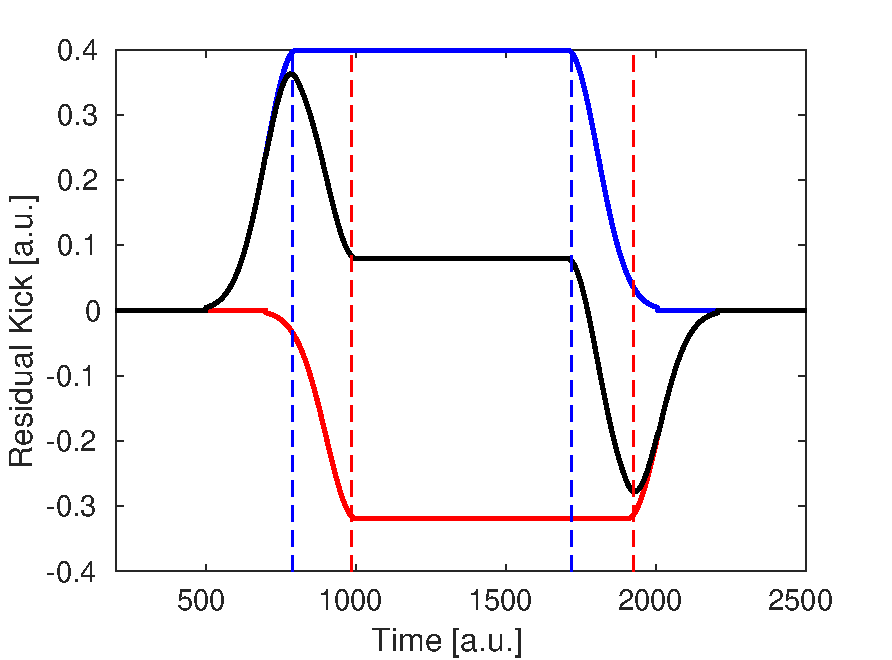
\includegraphics[width=0.6\columnwidth]{relDelay_sim}% Here is 
  %how to 
  %import EPS art
  \caption{\label{f:relDelay_sim} relDelay\_sim
  }
\end{figure}

The previous measurement verifies the timing of the correction signal applied 
to the first kicker (\(\mathrm{K_1}\)), which provides the phase shift in the 
chicane. The second kicker (\(\mathrm{K_2}\)) ensures the beam orbit downstream 
of the chicane is unaffected by the PFF correction, but has a negligible effect 
on the beam phase. The beam time of flight between the kickers is about 36~ns, 
thus the PFF correction voltage must arrive at \(\mathrm{K_2}\) 36~ns later 
than the correction at \(\mathrm{K_1}\). If this is not the case the PFF system 
will cause horizontal position offsets downstream of the chicane.

\begin{figure}
 \centering
  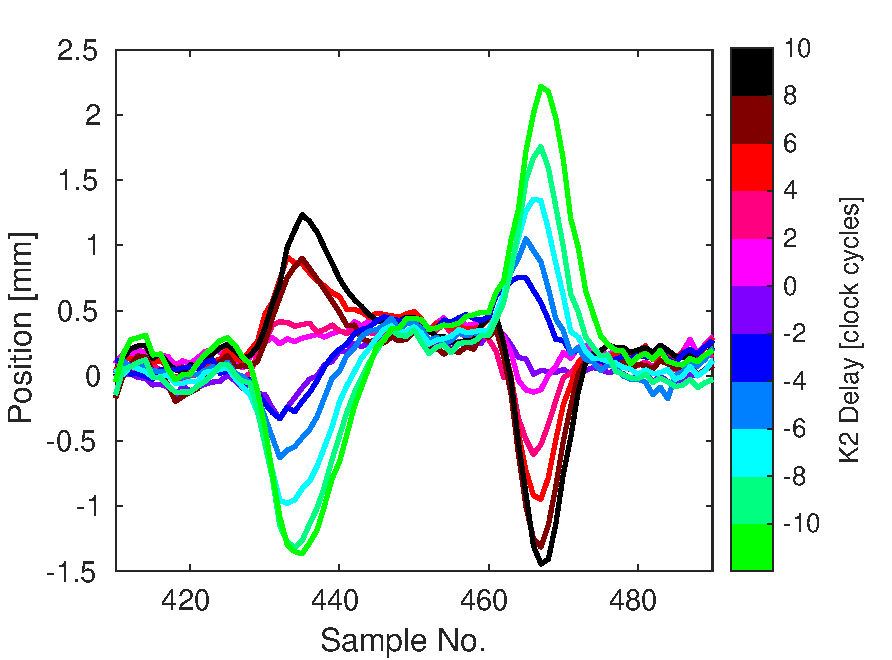
\includegraphics[width=0.6\columnwidth]{relDelay_traces}% Here is 
  %how to 
  %import EPS art
  \caption{\label{f:relDelay_traces}
  }
\end{figure}

Fig.~\ref{f:relDelay_sim} illustrates the effect of the 
correction not being synchronised with the beam at 
both kickers. A constant voltage is applied to the kickers, as shown in red and 
blue. The total kick, the sum of the two, is in black and should be zero for 
the whole pulse duration in the ideal PFF setup. A time offset between the 
kicker voltages with respect to the beam leads to a large residual kick at the 
start and end of the pulse. If the kicker voltages have different magnitudes 
there is also a constant offset in the central portion of the pulse.

\begin{figure}
 \centering
  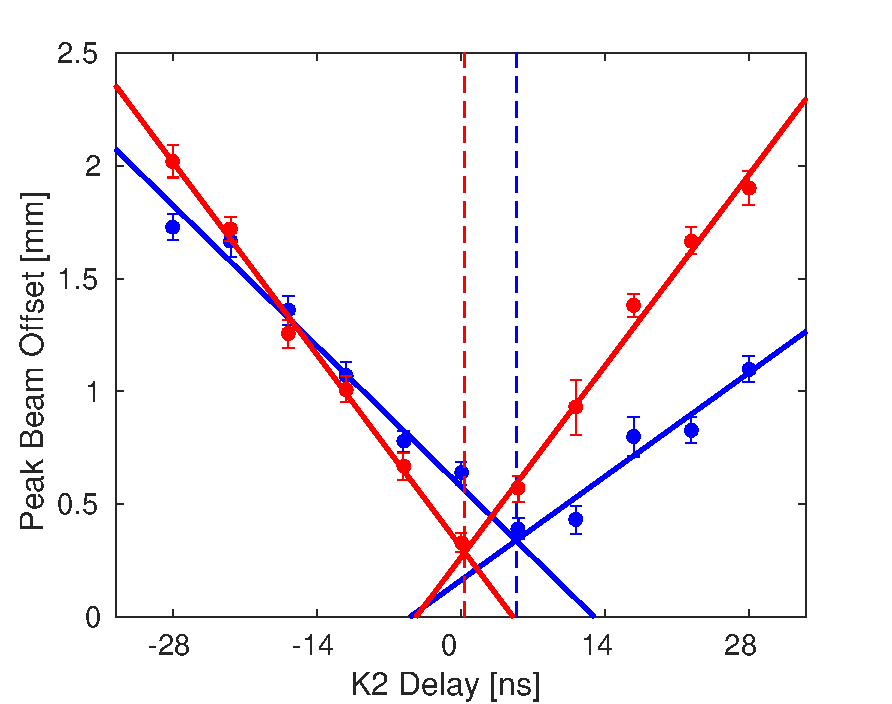
\includegraphics[width=0.6\columnwidth]{relDelay_fit}% Here is 
  \caption{\label{f:relDelay_fit}
  }
\end{figure}

The amplifier-to-kicker cables for \(K_2\) are longer than the \(K_1\) cables 
to compensate for additional beam time of flight. The 
correction output delay for each kicker can also be fine-tuned independently on 
the feedforward controller. 

To verify the timing of the \(K_2\) correction output the feedforward 
controller was used to apply a constant kick to a 168~ns portion of the pulse. 
The kick was applied in interleaved mode, with the horizontal position 
difference between the PFF Off and PFF On pulses measured in a BPM downstream 
of the chicane.
Fig.~\ref{f:relDelay_traces} shows this difference for different delays 
applied to the \(K_2\) correction output with respect to the \(K_1\) output, 
ranging from -28~ns to +28~ns. The response is similar to the simulated example 
in Fig.~\ref{f:relDelay_sim}, as expected.

The optimal delay for the \(K_2\) correction output minimises the size of the 
peaks resulting from residual kicks, and this is fitted for the peaks at both 
the leading and trailing end of the pulse in Fig.~\ref{f:relDelay_fit}. The 
fitted value is \(1.4\pm1.7\)~ns. During operation of the PFF system the 
\(K_2\) output was typically delayed by 2.8~ns with respect to \(K_1\). This is 
the minimum non-zero delay that can be applied by the feedforward controller 
(equivalent to one time period of the 357~MHz ADC clock frequency).

\subsection{\label{ss:gain}Correction Gain}

%PRL
\begin{figure}
 \centering
  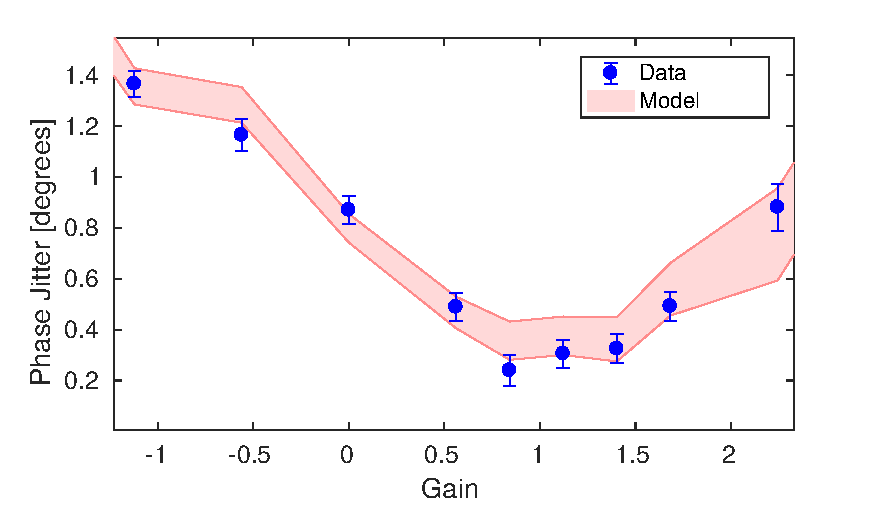
\includegraphics[width=0.6\columnwidth]{gScan}% Here is 
  \caption{\label{f:gScan}
  }
\end{figure}

The PFF system acts to remove the \(\phi_1\) phase, multiplied by a `gain' 
factor, from the phase at \(\phi_3\). If the phases at \(\phi_3\) and 
\(\phi_1\) are fully correlated, and the jitters are identical, the optimal 
system gain is unity.
In practice the gain is chosen to achieve optimal 
performance for real beam conditions. A representative gain scan is shown 
in~Fig.~\ref{fig:gScan}. The optimal gain is typically in the range 
0.9--1.3. Also shown in Fig.~\ref{fig:gScan} is a prediction of 
the corrected phase jitter at \(\phi_3\), using a simple model including the 
initial beam phase jitters at \(\phi_1\) and 
\(\phi_3\), the upstream-downstream phase correlation, and the gain 
\cite{RobertsThesis}. The model reproduces the data.
%/PRL

